% !TEX root = ../main.tex

\chapter{Deterministic approach}
\label{chap:Deterministic approach}

\section{Modeling approaches}

Problem as defined in section~\ref{sec:prob-def} can be reduced to two well known problems: transportation and min-cost max flow problem. In both cases from knowledge of $\mathbf{x}$ and constraint equations, $\mathbf{x}^{(h)}$ and $\mathbf{x}^{(b)}$ since at each $t$ in optimal solution at least one of $x^{(b)}_t$ and $x^{(h)}_t$ is $0$. This fact can easily be observed from flow conservation on intermediate nodes as in fig~\ref{fig:mcmf-model}. Setting them both to positive values create positive flow cycle with positive cost, which can be canceled yielding same flow with lower cost.

\subsection{Reduction to transportation problem}
\label{subs:trans}

For transportation problem reduction we need cost matrix for satisfying demand at time $j$ with supply at time $i$. It is given as follows:

\begin{definition}{$\mathbf{C}$}
matrix defines cost for satisfying demand with specific raw supply material purchase date. It's element $c_{ij}$ equals:

\begin{equation*}
    c_{ij} = \begin{cases}
        b \left( i - j \right) + s_i & j < i \\
        h \left( j - i \right) + s_i & j \ge i
    \end{cases}
\end{equation*}
That is using raw materials purchased at $i$ to satisfy demand at time $j$ incurs cost $c_{ij}$.
\end{definition}

Maximum supply $\mathbf{x^{(\max)}}$ is given, so is the demand vector $\mathbf{d}$. Since transportation problem required equal supply and demand nodes, we add a dummy demand node consuming excess supply.
\unsure{"That is 0 in the deterministic..." I don't understand what is the meaning of this remark and how can implement your feedback.}

Transportation problem~\autocite{or-textbook} is easy reduction since we have cost matrix $\mathbf{C}$ defining ``transportation'' costs associated with each possible assignment option. For successful reduction we only need adding dummy source or destination.

\subsection{Min cost max flow reduction}
\label{sub:Min cost max flow reduction}

We can exploit additional problem structure to achieve superior performance and modeling capabilities. In figure~\ref{fig:mcmf-model} we see network architecture.

\begin{figure}[h]
\label{fig:mcmf-model}
  \centering
  
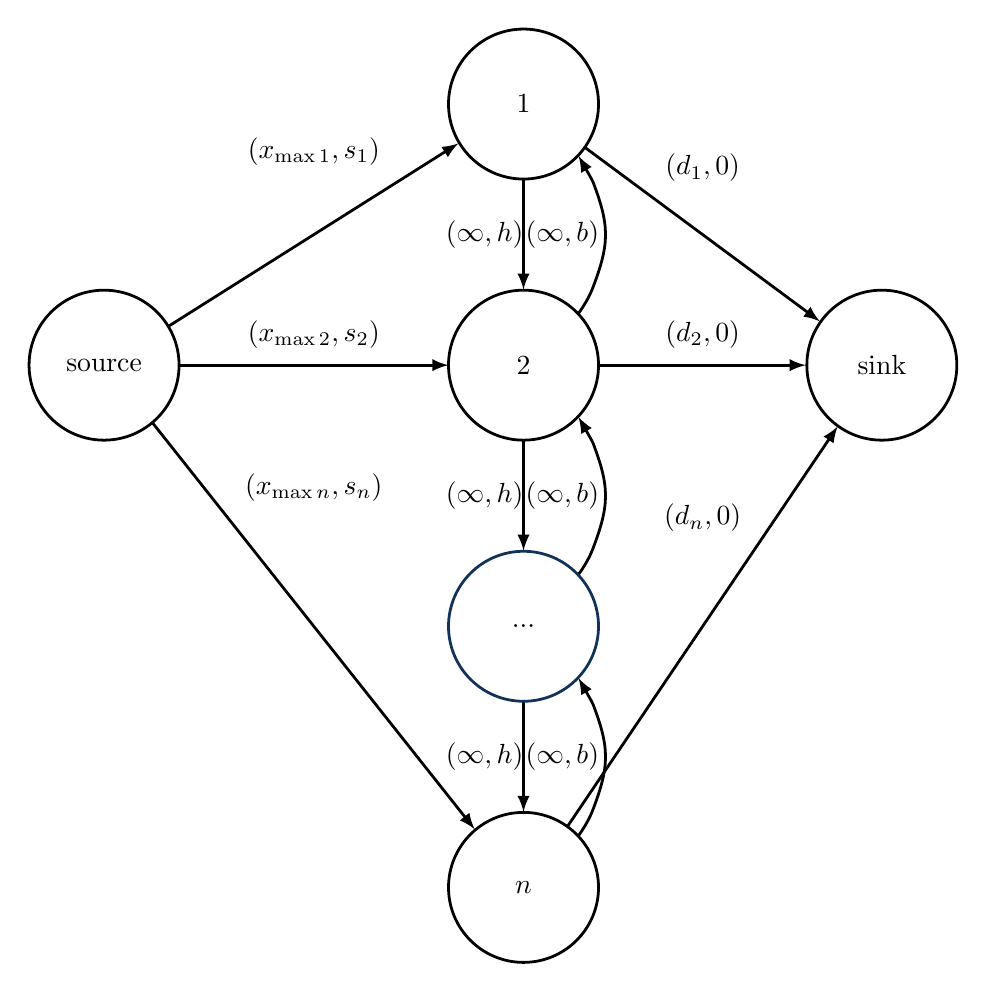
\begin{tikzpicture}[>=latex,line join=bevel,]
  \pgfsetlinewidth{1bp}
%%
\begin{scope}
  \pgfsetstrokecolor{black}
  \definecolor{strokecol}{rgb}{1.0,1.0,1.0};
  \pgfsetstrokecolor{strokecol}
  \definecolor{fillcol}{rgb}{1.0,1.0,1.0};
  \pgfsetfillcolor{fillcol}
  \filldraw (0.0bp,0.0bp) -- (0.0bp,336.0bp) -- (334.0bp,336.0bp) -- (334.0bp,0.0bp) -- cycle;
\end{scope}
\begin{scope}
  \pgfsetstrokecolor{black}
  \definecolor{strokecol}{rgb}{1.0,1.0,1.0};
  \pgfsetstrokecolor{strokecol}
  \definecolor{fillcol}{rgb}{1.0,1.0,1.0};
  \pgfsetfillcolor{fillcol}
  \filldraw (0.0bp,0.0bp) -- (0.0bp,336.0bp) -- (334.0bp,336.0bp) -- (334.0bp,0.0bp) -- cycle;
\end{scope}
  \pgfsetcolor{black}
  % Edge: n -> m
  \draw [->] (197.79bp,45.647bp) .. controls (199.91bp,48.565bp) and (201.75bp,51.712bp)  .. (203.0bp,55.0bp) .. controls (209.02bp,70.78bp) and (209.02bp,77.22bp)  .. (203.0bp,93.0bp) .. controls (202.92bp,93.205bp) and (202.84bp,93.41bp)  .. (197.79bp,102.35bp);
  \definecolor{strokecol}{rgb}{0.0,0.0,0.0};
  \pgfsetstrokecolor{strokecol}
  \draw (192.0bp,74.0bp) node {$(\infty, b)$};
  \draw (203.79bp,51.647bp) node {$$};
  \draw (203.79bp,96.353bp) node {$$};
  % Edge: m -> n
  \draw [->] (178.0bp,93.872bp) .. controls (178.0bp,84.622bp) and (178.0bp,74.113bp)  .. (178.0bp,54.189bp);
  \draw (164.0bp,74.0bp) node {$(\infty, h)$};
  \draw (184.0bp,90.872bp) node {$$};
  \draw (184.0bp,54.189bp) node {$$};
  % Edge: source -> 2
  \draw [->] (54.295bp,215.0bp) .. controls (78.339bp,215.0bp) and (114.12bp,215.0bp)  .. (150.97bp,215.0bp);
  \draw (102.5bp,226.0bp) node {$(x_{\max 2}, s_2)$};
  \draw (60.295bp,209.0bp) node {$$};
  \draw (144.97bp,209.0bp) node {$$};
  % Edge: 2 -> 1
  \draw [->] (197.79bp,233.65bp) .. controls (199.91bp,236.57bp) and (201.75bp,239.71bp)  .. (203.0bp,243.0bp) .. controls (209.02bp,258.78bp) and (209.02bp,265.22bp)  .. (203.0bp,281.0bp) .. controls (202.92bp,281.21bp) and (202.84bp,281.41bp)  .. (197.79bp,290.35bp);
  \draw (192.0bp,262.0bp) node {$(\infty, b)$};
  \draw (203.79bp,239.65bp) node {$$};
  \draw (191.79bp,284.35bp) node {$$};
  % Edge: n -> sink
  \draw [->] (193.82bp,48.934bp) .. controls (216.41bp,82.381bp) and (259.56bp,146.25bp)  .. (291.08bp,192.92bp);
  \draw (242.5bp,160.0bp) node {$(d_n, 0)$};
  \draw (187.82bp,42.934bp) node {$$};
  \draw (285.08bp,186.92bp) node {$$};
  % Edge: m -> 2
  \draw [->] (197.79bp,139.65bp) .. controls (199.91bp,142.57bp) and (201.75bp,145.71bp)  .. (203.0bp,149.0bp) .. controls (209.02bp,164.78bp) and (209.02bp,171.22bp)  .. (203.0bp,187.0bp) .. controls (202.92bp,187.21bp) and (202.84bp,187.41bp)  .. (197.79bp,196.35bp);
  \draw (192.0bp,168.0bp) node {$(\infty, b)$};
  \draw (203.79bp,145.65bp) node {$$};
  \draw (203.79bp,190.35bp) node {$$};
  % Edge: 2 -> m
  \draw [->] (178.0bp,187.87bp) .. controls (178.0bp,178.62bp) and (178.0bp,168.11bp)  .. (178.0bp,148.19bp);
  \draw (164.0bp,168.0bp) node {$(\infty, h)$};
  \draw (184.0bp,184.87bp) node {$$};
  \draw (184.0bp,148.19bp) node {$$};
  % Edge: 1 -> sink
  \draw [->] (200.26bp,293.27bp) .. controls (221.14bp,277.81bp) and (253.17bp,254.1bp)  .. (284.67bp,230.78bp);
  \draw (242.5bp,286.0bp) node {$(d_1, 0)$};
  \draw (206.26bp,287.27bp) node {$$};
  \draw (278.67bp,224.78bp) node {$$};
  % Edge: 1 -> 2
  \draw [->] (178.0bp,281.87bp) .. controls (178.0bp,272.62bp) and (178.0bp,262.11bp)  .. (178.0bp,242.19bp);
  \draw (164.0bp,262.0bp) node {$(\infty, h)$};
  \draw (184.0bp,281.87bp) node {$$};
  \draw (184.0bp,245.19bp) node {$$};
  % Edge: source -> n
  \draw [->] (44.515bp,194.16bp) .. controls (71.142bp,160.57bp) and (123.63bp,94.338bp)  .. (160.41bp,47.931bp);
  \draw (102.5bp,171.0bp) node {$(x_{\max n}, s_n)$};
  \draw (50.515bp,188.16bp) node {$$};
  \draw (154.41bp,53.931bp) node {$$};
  % Edge: source -> 1
  \draw [->] (50.307bp,229.07bp) .. controls (75.653bp,245.06bp) and (117.2bp,271.27bp)  .. (154.54bp,294.83bp);
  \draw (102.5bp,292.0bp) node {$(x_{\max 1}, s_1)$};
  \draw (56.307bp,223.07bp) node {$$};
  \draw (148.54bp,288.83bp) node {$$};
  % Edge: 2 -> sink
  \draw [->] (205.01bp,215.0bp) .. controls (223.63bp,215.0bp) and (248.96bp,215.0bp)  .. (279.59bp,215.0bp);
  \draw (242.5bp,226.0bp) node {$(d_2, 0)$};
  \draw (211.01bp,209.0bp) node {$$};
  \draw (273.59bp,209.0bp) node {$$};
  % Node: m
\begin{scope}
  \definecolor{strokecol}{rgb}{0.07,0.2,0.34};
  \pgfsetstrokecolor{strokecol}
  \draw (178.0bp,121.0bp) ellipse (27.0bp and 27.0bp);
  \definecolor{strokecol}{rgb}{0.0,0.0,0.0};
  \pgfsetstrokecolor{strokecol}
  \draw (178.0bp,121.0bp) node {$...$};
\end{scope}
  % Node: n
\begin{scope}
  \definecolor{strokecol}{rgb}{0.0,0.0,0.0};
  \pgfsetstrokecolor{strokecol}
  \draw (178.0bp,27.0bp) ellipse (27.0bp and 27.0bp);
  \draw (178.0bp,27.0bp) node {$n$};
\end{scope}
  % Node: 1
\begin{scope}
  \definecolor{strokecol}{rgb}{0.0,0.0,0.0};
  \pgfsetstrokecolor{strokecol}
  \draw (178.0bp,309.0bp) ellipse (27.0bp and 27.0bp);
  \draw (178.0bp,309.0bp) node {$1$};
\end{scope}
  % Node: source
\begin{scope}
  \definecolor{strokecol}{rgb}{0.0,0.0,0.0};
  \pgfsetstrokecolor{strokecol}
  \draw (27.0bp,215.0bp) ellipse (27.0bp and 27.0bp);
  \draw (27.0bp,215.0bp) node {source};
\end{scope}
  % Node: 2
\begin{scope}
  \definecolor{strokecol}{rgb}{0.0,0.0,0.0};
  \pgfsetstrokecolor{strokecol}
  \draw (178.0bp,215.0bp) ellipse (27.0bp and 27.0bp);
  \draw (178.0bp,215.0bp) node {$2$};
\end{scope}
  % Node: sink
\begin{scope}
  \definecolor{strokecol}{rgb}{0.0,0.0,0.0};
  \pgfsetstrokecolor{strokecol}
  \draw (307.0bp,215.0bp) ellipse (27.0bp and 27.0bp);
  \draw (307.0bp,215.0bp) node {sink};
\end{scope}
%
\end{tikzpicture}


  \caption{min cost max flow model. Arcs are labeled (capacity, cost)}
\end{figure}

\subsection{Runtime complexity}

Since both transportation problem and min-cost max flow have polynomial solution algorithms~\autocite{or-textbook}~\autocite{Orlin1997}, this problem does too. Most efficient approach is using network simplex since this problem naturally fits into min-cost max flow model than reduction to transportation problem.

\section{Variants}
\label{sec:Variants}

Problem as defined previously could seem rather simplistic and not allowing useful extensions users might want, such as starting storage amount and similar. In following few subsections most useful extensions are described.

\subsection{Starting storage capacity}
In case we already have a certain number of product in stock we can easily embed that knowledge into the model by setting $x^{(h)}_0$ equal to starting storage capacity

\subsection{Ending storage requirement}
\label{subs:Ending storage requirement}
For example we'd like to have some extra product in stock by the end of analysis, and it's quite easy to accommodate such requirement. Simple set $x^{(h)}_n$ to ending requirements. In min-cost max flow model that would be equivalent to another arch from node $n$ to sink with ending storage requirement capacity.

\subsection{Allowing future backlogging}
\label{subs:Allowing future backlogging}
In the model as described, time stops at period $n$, however, in realistic scenario we're looking at only short time snapshot of ongoing process. Simplest modification would be allowing $x^{(b)}_n$ to be non-negative and letting it be decision variable. It's value is going to be amount of backlogged demand at the analysis end, that is time $n$.

\subsection{Leap time ordering}
\label{subs:leap-time-ordering}
If we order raw materials at $t$ they might arrive at later time moment $t+\Delta_t$. This can easily be modeled via variable substitution. For different $\Delta_t$ depending on the $t$ or multiple suppliers see Subsection~\ref{subs:Multiple raw material suppliers}

\subsection{Multiple raw material suppliers}
\label{subs:Multiple raw material suppliers}
Adding new raw material suppliers with different costs cannot be done as per original model specification. Talking in terms or min-cost max flow approach adding new raw material suppliers would be equal to adding additional arcs from source to nodes 1, 2, \ldots, $n$. with respective maximum supply capacity and costs.
